\chapter{Network Editors}
\label{ch:networkeditor}
% ##################################################################################################################

\hfill \textbf{Authors:} Andreas Neumann, Michael Zilske, Sergio Arturo Ordóñez

\begin{center} 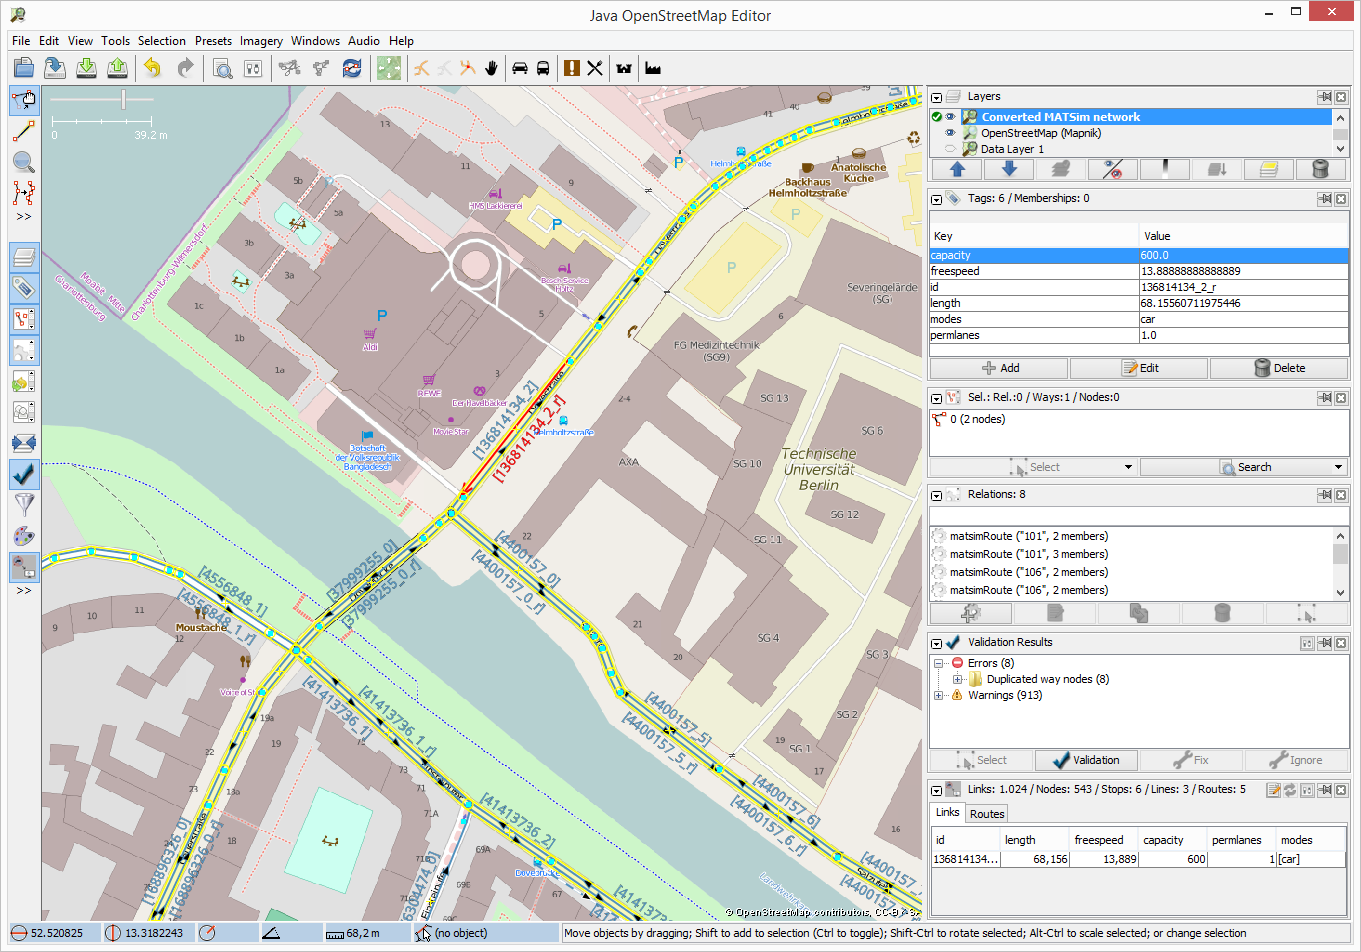
\includegraphics[width=0.4\textwidth, angle=0]{extending/figures/networkeditor/josm_screenshot} \end{center}

\createStandardInformationBasic{networkEditor}{start the plugin from JOSM directly}{todo}{todo}

% ##################################################################################################################
\section{MATSim JOSM Network Editor}
A plugin for the \gls{josm} \citep[][]{JOSM2014}, is available simplifying the process of creating and editing \gls{matsim} networks. This plugin fully integrates with \gls{josm} and thus benefits from its build-in functionality.
%
% -------------------
\createfigure
{JOSM with converted MATSim network and \protect\gls{osm} background imagery}
{JOSM with converted MATSim network and \protect\gls{osm} background imagery. Map data taken from \citet[][]{OpenStreetMap2014}}
{\label{fig:networkeditor_screenshot}}
{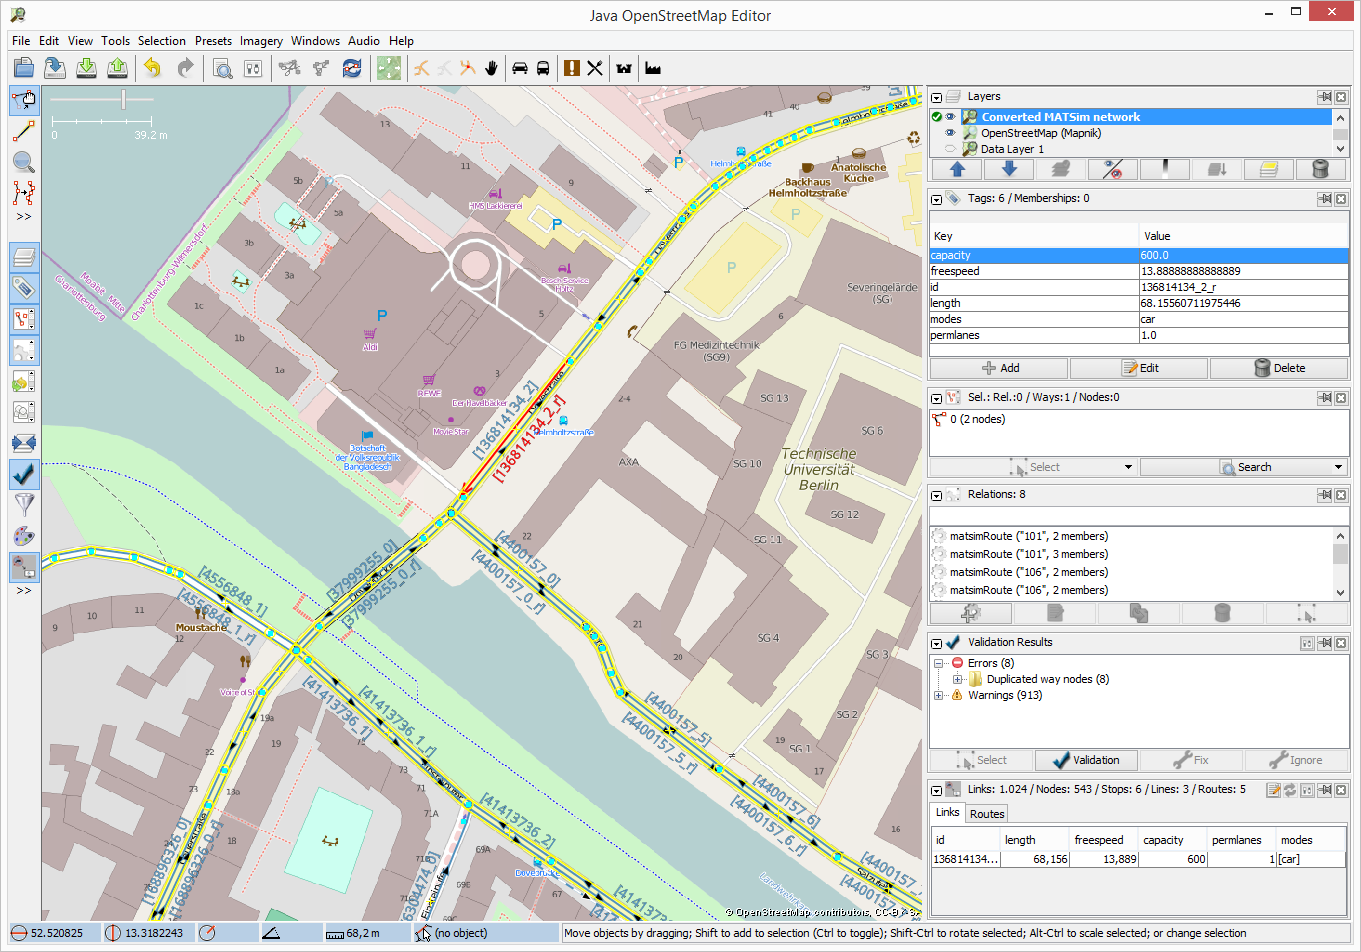
\includegraphics[width=1.0\textwidth]{extending/figures/networkeditor/josm_screenshot}}
{}
% -------------------

% ===========================================================================================
\subsection{Features}
The \gls{matsim} \gls{josm} lets you preview, edit and save a \gls{matsim} network directly from the map. Basic support for converting and editing public transport networks is implemented. The plug-in allows to automatically post-process a network by removing unnecessary intermediate nodes and links.
\begin{description}\styleDescription
\item[Convert] \gls{matsim} networks from \gls{osm}. Load map data for a selected area directly from the Internet or load it from a local \gls{osm} file. Specify conversion parameters and save a \gls{matsim} network.
\item[Visualize] an existing or newly converted \gls{matsim} network along with other data like satellite imagery or other \gls{josm}-supported layers.
\item[Edit] an existing or newly converted \gls{matsim} network with the available \gls{josm} tools you know. Use the build-in undo and search functions of \gls{josm}. Changes to the underlying \gls{osm} data are instantly reflected by the converted \gls{matsim} network. Use \gls{matsim}-specific presets to minimize errors.
\item[Validate] an existing or newly converted \gls{matsim} network with respect to the requirements of the \gls{matsim} network file description. Visualize the errors and fix them (automatically). 
\end{description}
The next version will support public transport networks.

% ===========================================================================================
\subsection{Installing the Plug-In}
You do not need to download the source to use it. It is in the \gls{josm} plug-in repository. Just start \gls{josm} and look for the \gls{matsim} plug-in under \lstinline|Edit...Preferences...Plugins|. Download the list of available plug-ins and search for ``matsim''. Tick the box, press \lstinline|ok| and restart \gls{josm}.

% ===========================================================================================
\subsection{Getting the Code}
The source code is hosted on github (\url{https://github.com/matsim-org/josm-matsim-plugin}). Unlike \gls{matsim}, the build is not based on \gls{maven}, but on Gradle. Editing the \lstinline|Manifest|, downloading \gls{josm} for compilation, and building a flat \gls{jar} are easier in Gradle. Use your favorite \gls{ide} to import the Gradle project and/or see the comments in \lstinline|build.gradle| for details. You can run \gls{josm} and the plug-in in the debugger.
 
% ##################################################################################################################
\section{Map-to-Map Matching Editors in Singapore}
\label{sec:networkeditor-singapore}
For the Singapore scenario, and concerning the supply data, a high resolution network was obtained from the \gls{navteq} company. These network consists of a graph which represent every road in the island, which results very convenient for a high resolution model like \gls{matsim}. However, the information of travel capacities and free speeds of the network links is not accurate. On the other hand, local authorities provided the network model used for planning. This network does not represent minor roads and intersections are simplified, but capacities and free speed are accurately estimated. Figure~\ref{fig:Capacities} shows lower travel capacities of many primary roads in the navigation model (right) than in the planning model (left).

% -------------------
\createfigure
{Difference in the travel capacities}
{Difference in the travel capacities between the planning network model of Singapore (left) and a navigation network model (right)}
{\label{fig:Capacities}}
{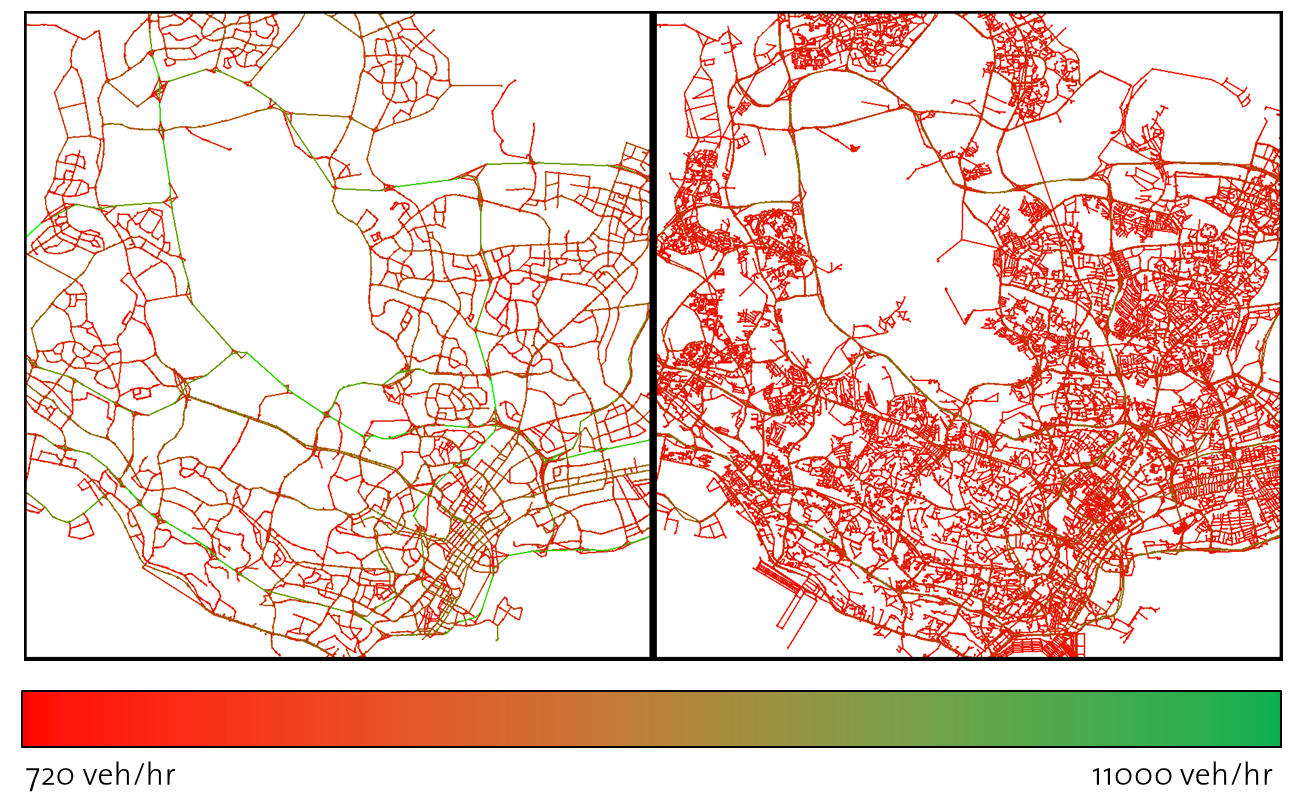
\includegraphics[width=1.0\textwidth]{extending/figures/netEdSing/Capacities.png}}
{}
% -------------------

This section describes a semi-automatic tool developed to match these two network models \citep[][]{Ordonez_Webpage_2011_3}. Thus, the capacities and free speeds of the main links of the navigation network (high-res network) can be updated with the ones of the planning network (low-res network).

% ===========================================================================================
\subsection{General Procedure}
Although many authors focus on try to solve the matching problem of two networks in a formal way, this work follows a semi-automatic approach. This means that automatic algorithms will try to solve the problem, but the user knows the solution won't be perfect and some manual work is expected to be done. Hence, interactive tools are also provided to the user to manually improve the solutions.

The map-to-map procedure is based on the algorithm developed by \citet{BalmerEtAl_STRC_2005}. It consists of the following steps:
%
\begin{enumerate}\styleEnumerate
\item Classify the nodes according to their topology (\eg source, sink, one way start, crossing) in both networks.
\item Reduce the networks according to the previous classification, and saving the relations to the original nodes.
\item Find crossings (set of close nodes) in both networks and relate them.
\item \textbf{Assuming not all crossings were found in the previous step, use the interactive tool shown in the Figure~\ref{fig:Nodes} to find all the crossings in both networks and relate them}
\item Recognize links or sequences of links which join the crossings found in (3) and (4)
\item \textbf{Assuming not all links or paths found in the previous step are correct, use the link-link matching interactive tool shown in the Figure~\ref{fig:Links}, to find or modify links or sequences of links which join the crossings}
\item Update capacities and free speeds of the matched links found in (5) and (6)
\end{enumerate}
%
\createfigure
{Crossing-crossing matching application}
{Crossing-crossing matching application. A second node, matching the pink node o the low-res network on the left, is being selected from the high-res network on the right}
{\label{fig:Nodes}}
{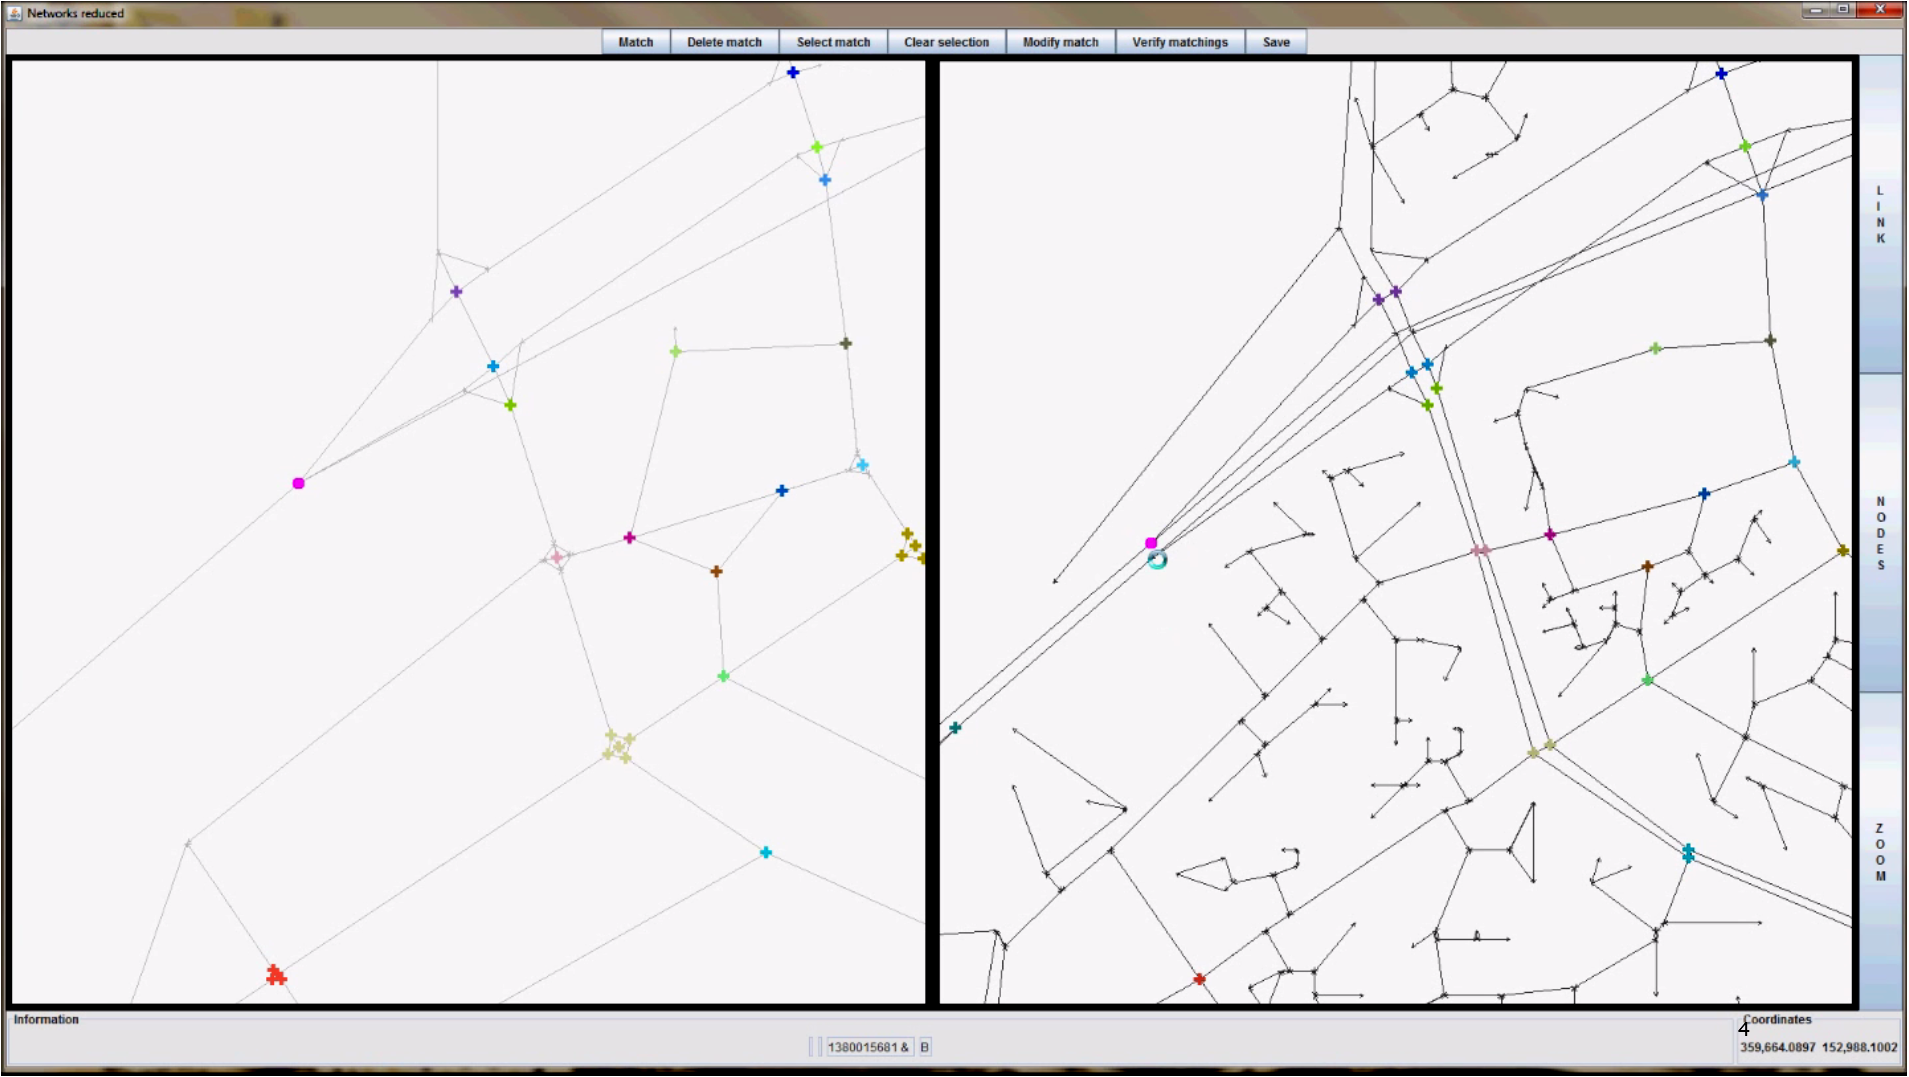
\includegraphics[width=1.0\textwidth]{extending/figures/netEdSing/Nodes.png}}
{}

% ===========================================================================================
\subsection{Interactive Tools Characteristics}
As shown in Figure~\ref{fig:Nodes} the application allows to interactively modify crossing-crossing relationships. A very similar interactive tool was develop to also modify link-link relationships between the high resolution network and the low resolution one. They can be found at the package \lstinline|playground.sergioo.networksMatcher2012| in the playgrounds project of \gls{matsim}. To run the graphic interface of the crossings-crossing application use the class \lstinline|gui.DoubleNetworkMatchingWindow|, and use the class \lstinline|gui.DoubleNetworkCapacitiesWindow| for the link-link application. These applications write simple text files of the relationships found. The program found at the class \lstinline|ApplyCapacities| overwrites the capacities and/or free speeds according to the simple text files, and writes the new \gls{xml} file of the resulting network. This multiple-steps design allows to run the interactive applications several times or in parallel. Developed functional requirements and quality attributes of the interactive tools are described as follows:
%
\createfigure
{Link-link matching application}
{Link-link matching application. A shortest path algorithm to select a sequence of links of the network on the right will be executed when clicking the destination node}
{\label{fig:Links}}
{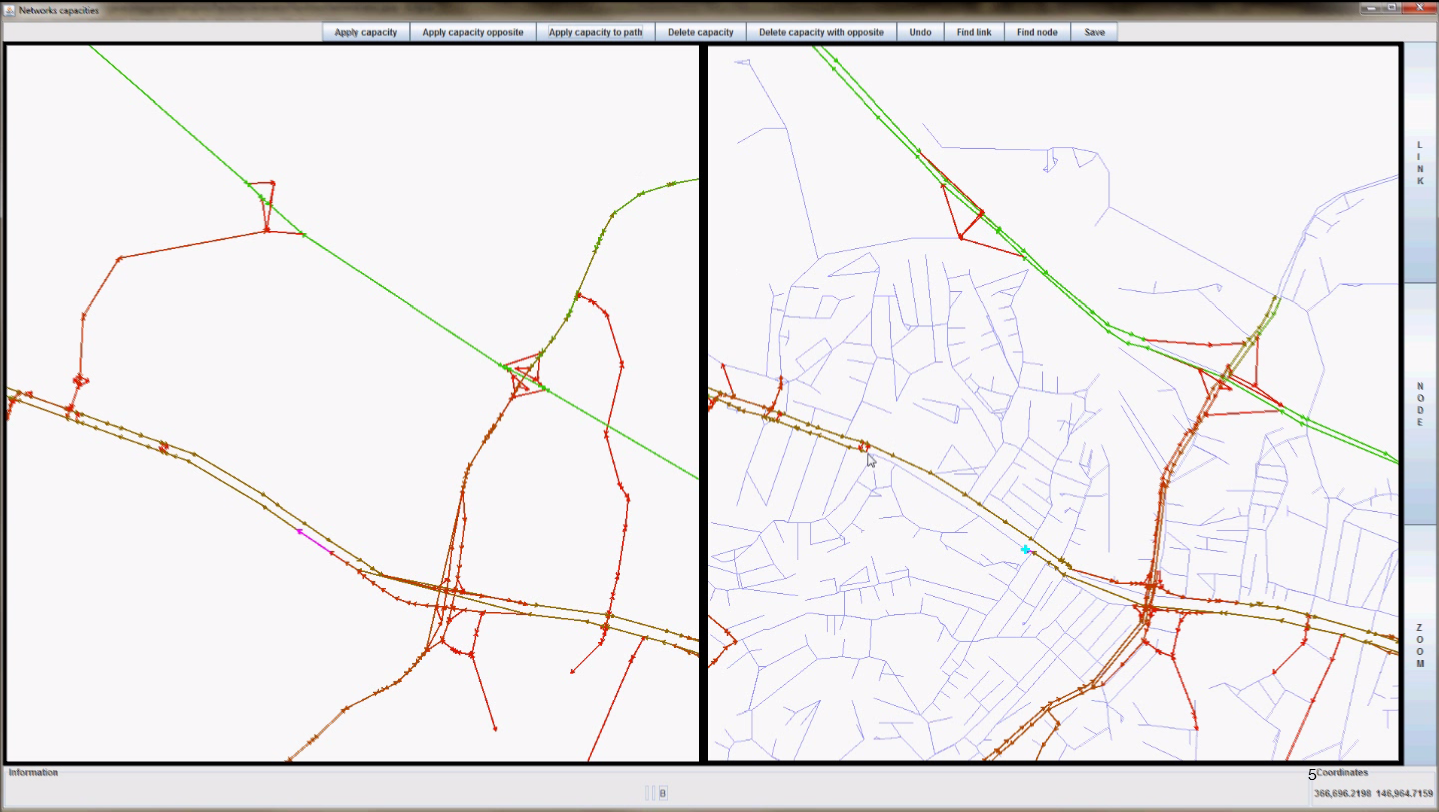
\includegraphics[width=1.0\textwidth]{extending/figures/netEdSing/Links.png}}
{}

\begin{itemize}\styleItemize
\item Visualization: Two navigation networks are displayed in two modes. The first mode splits the window in two, showing each network at one side and maintaining them at the same geographical position and zoom when navigating. The second superimposes both networks in the same window, but only one is active. Selected elements are drawn in different colors. Everything is displayed in a bi-dimensional interactive way, displaying the location of the cursor in the working coordinates, and including panning, zoom and view-all options. The crossing-crossing application displays matched set of nodes (crossings) with the same color in both networks. The link-link application tool also allows to visualize the value of the capacity property (or the free speed property) of the links in both networks using a color scale, as shown in Figure~\ref{fig:Links}.
\item Selection: The applications allow to select links and nodes from both networks. The crossing-crossing one just allows to select set of nodes. The link-link application allows to select sequence of links. This can be do directly or selecting an origin node, a destination node and running a ``select shortest path algorithm tool''. It is also possible to select the opposite link to the one which is selected.
\item Matching and Deletion: The applications allow to create a similarity relationship between the elements selected in both networks, set of nodes or sequence of links.
\item Saving: The applications allow to save the relationships found.
\item Loading: The applications allow to load previous relationships found.
\item Others: The crossing-crossing application executes and automatic verification of the currently found matching, to avoid repeated nodes. It also allows to clear the current selection. The link-link application allows to automatically navigate to a link or node specified by the user using its id. It also allows to undo previous matching. 
\end{itemize}

% ===========================================================================================
\subsection{Results}
All the links of the low-res network were matched to links of the high-res network, updating the corresponding link properties. Figure~\ref{fig:Results} shows the differences in travel capacities between the original navigation network values and the final version. Eight hours of manual work was necessary to match crossings and ten hours of manual work was necessary to match links. Obviously, improvements in the accuracy and completeness of the automatic matching algorithms reduce the manual work time.
%
\createfigure
{Resulting changes in the travel capacity property of the navigation network}
{Resulting changes in the travel capacity property of the navigation network}
{\label{fig:Results}}
{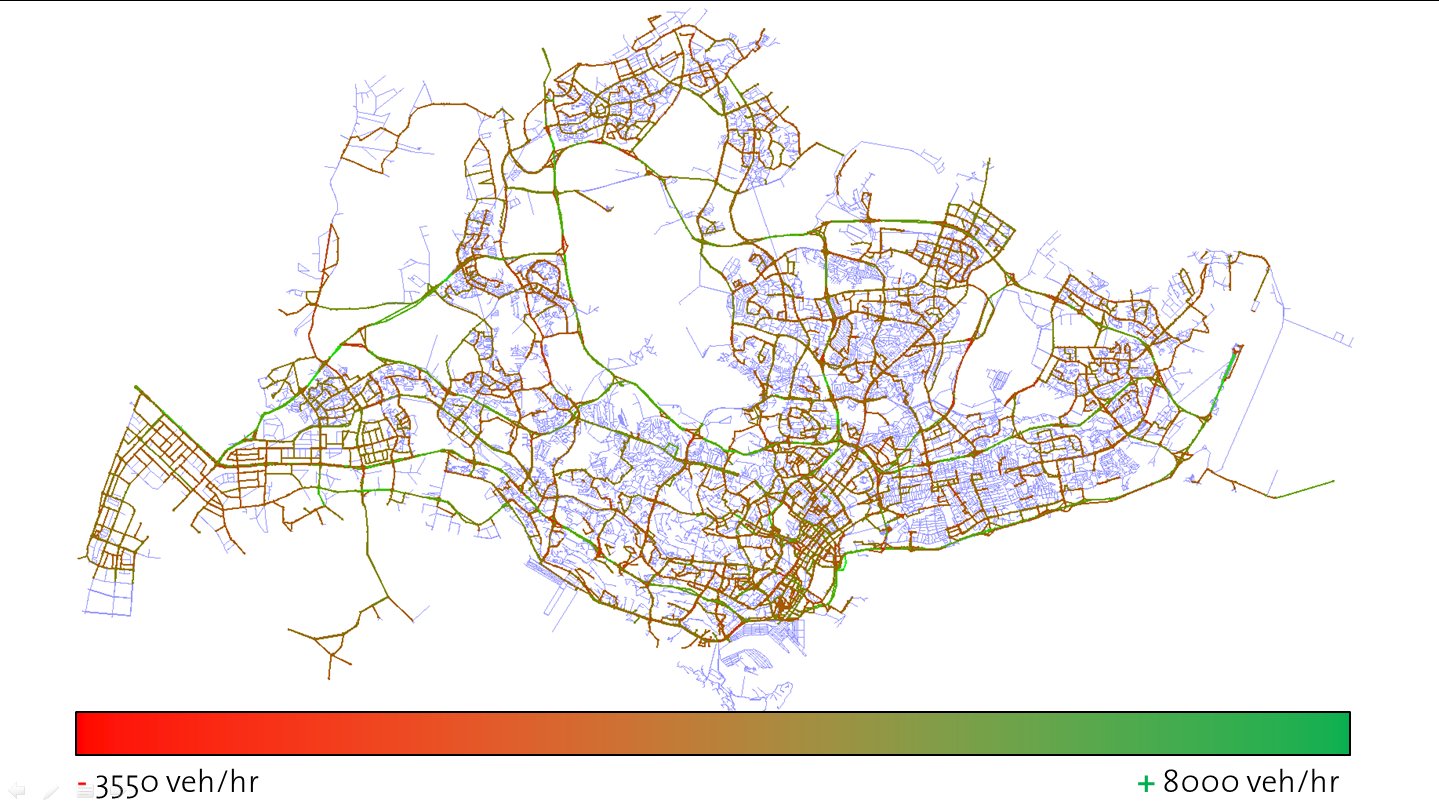
\includegraphics[width=1.0\textwidth]{extending/figures/netEdSing/Result.png}}
{}

% ##################################################################################################################
